% Options for packages loaded elsewhere
\PassOptionsToPackage{unicode}{hyperref}
\PassOptionsToPackage{hyphens}{url}
%
\documentclass[
]{book}
\usepackage{amsmath,amssymb}
\usepackage{iftex}
\ifPDFTeX
  \usepackage[T1]{fontenc}
  \usepackage[utf8]{inputenc}
  \usepackage{textcomp} % provide euro and other symbols
\else % if luatex or xetex
  \usepackage{unicode-math} % this also loads fontspec
  \defaultfontfeatures{Scale=MatchLowercase}
  \defaultfontfeatures[\rmfamily]{Ligatures=TeX,Scale=1}
\fi
\usepackage{lmodern}
\ifPDFTeX\else
  % xetex/luatex font selection
\fi
% Use upquote if available, for straight quotes in verbatim environments
\IfFileExists{upquote.sty}{\usepackage{upquote}}{}
\IfFileExists{microtype.sty}{% use microtype if available
  \usepackage[]{microtype}
  \UseMicrotypeSet[protrusion]{basicmath} % disable protrusion for tt fonts
}{}
\makeatletter
\@ifundefined{KOMAClassName}{% if non-KOMA class
  \IfFileExists{parskip.sty}{%
    \usepackage{parskip}
  }{% else
    \setlength{\parindent}{0pt}
    \setlength{\parskip}{6pt plus 2pt minus 1pt}}
}{% if KOMA class
  \KOMAoptions{parskip=half}}
\makeatother
\usepackage{xcolor}
\usepackage{color}
\usepackage{fancyvrb}
\newcommand{\VerbBar}{|}
\newcommand{\VERB}{\Verb[commandchars=\\\{\}]}
\DefineVerbatimEnvironment{Highlighting}{Verbatim}{commandchars=\\\{\}}
% Add ',fontsize=\small' for more characters per line
\usepackage{framed}
\definecolor{shadecolor}{RGB}{248,248,248}
\newenvironment{Shaded}{\begin{snugshade}}{\end{snugshade}}
\newcommand{\AlertTok}[1]{\textcolor[rgb]{0.94,0.16,0.16}{#1}}
\newcommand{\AnnotationTok}[1]{\textcolor[rgb]{0.56,0.35,0.01}{\textbf{\textit{#1}}}}
\newcommand{\AttributeTok}[1]{\textcolor[rgb]{0.13,0.29,0.53}{#1}}
\newcommand{\BaseNTok}[1]{\textcolor[rgb]{0.00,0.00,0.81}{#1}}
\newcommand{\BuiltInTok}[1]{#1}
\newcommand{\CharTok}[1]{\textcolor[rgb]{0.31,0.60,0.02}{#1}}
\newcommand{\CommentTok}[1]{\textcolor[rgb]{0.56,0.35,0.01}{\textit{#1}}}
\newcommand{\CommentVarTok}[1]{\textcolor[rgb]{0.56,0.35,0.01}{\textbf{\textit{#1}}}}
\newcommand{\ConstantTok}[1]{\textcolor[rgb]{0.56,0.35,0.01}{#1}}
\newcommand{\ControlFlowTok}[1]{\textcolor[rgb]{0.13,0.29,0.53}{\textbf{#1}}}
\newcommand{\DataTypeTok}[1]{\textcolor[rgb]{0.13,0.29,0.53}{#1}}
\newcommand{\DecValTok}[1]{\textcolor[rgb]{0.00,0.00,0.81}{#1}}
\newcommand{\DocumentationTok}[1]{\textcolor[rgb]{0.56,0.35,0.01}{\textbf{\textit{#1}}}}
\newcommand{\ErrorTok}[1]{\textcolor[rgb]{0.64,0.00,0.00}{\textbf{#1}}}
\newcommand{\ExtensionTok}[1]{#1}
\newcommand{\FloatTok}[1]{\textcolor[rgb]{0.00,0.00,0.81}{#1}}
\newcommand{\FunctionTok}[1]{\textcolor[rgb]{0.13,0.29,0.53}{\textbf{#1}}}
\newcommand{\ImportTok}[1]{#1}
\newcommand{\InformationTok}[1]{\textcolor[rgb]{0.56,0.35,0.01}{\textbf{\textit{#1}}}}
\newcommand{\KeywordTok}[1]{\textcolor[rgb]{0.13,0.29,0.53}{\textbf{#1}}}
\newcommand{\NormalTok}[1]{#1}
\newcommand{\OperatorTok}[1]{\textcolor[rgb]{0.81,0.36,0.00}{\textbf{#1}}}
\newcommand{\OtherTok}[1]{\textcolor[rgb]{0.56,0.35,0.01}{#1}}
\newcommand{\PreprocessorTok}[1]{\textcolor[rgb]{0.56,0.35,0.01}{\textit{#1}}}
\newcommand{\RegionMarkerTok}[1]{#1}
\newcommand{\SpecialCharTok}[1]{\textcolor[rgb]{0.81,0.36,0.00}{\textbf{#1}}}
\newcommand{\SpecialStringTok}[1]{\textcolor[rgb]{0.31,0.60,0.02}{#1}}
\newcommand{\StringTok}[1]{\textcolor[rgb]{0.31,0.60,0.02}{#1}}
\newcommand{\VariableTok}[1]{\textcolor[rgb]{0.00,0.00,0.00}{#1}}
\newcommand{\VerbatimStringTok}[1]{\textcolor[rgb]{0.31,0.60,0.02}{#1}}
\newcommand{\WarningTok}[1]{\textcolor[rgb]{0.56,0.35,0.01}{\textbf{\textit{#1}}}}
\usepackage{longtable,booktabs,array}
\usepackage{calc} % for calculating minipage widths
% Correct order of tables after \paragraph or \subparagraph
\usepackage{etoolbox}
\makeatletter
\patchcmd\longtable{\par}{\if@noskipsec\mbox{}\fi\par}{}{}
\makeatother
% Allow footnotes in longtable head/foot
\IfFileExists{footnotehyper.sty}{\usepackage{footnotehyper}}{\usepackage{footnote}}
\makesavenoteenv{longtable}
\usepackage{graphicx}
\makeatletter
\def\maxwidth{\ifdim\Gin@nat@width>\linewidth\linewidth\else\Gin@nat@width\fi}
\def\maxheight{\ifdim\Gin@nat@height>\textheight\textheight\else\Gin@nat@height\fi}
\makeatother
% Scale images if necessary, so that they will not overflow the page
% margins by default, and it is still possible to overwrite the defaults
% using explicit options in \includegraphics[width, height, ...]{}
\setkeys{Gin}{width=\maxwidth,height=\maxheight,keepaspectratio}
% Set default figure placement to htbp
\makeatletter
\def\fps@figure{htbp}
\makeatother
\setlength{\emergencystretch}{3em} % prevent overfull lines
\providecommand{\tightlist}{%
  \setlength{\itemsep}{0pt}\setlength{\parskip}{0pt}}
\setcounter{secnumdepth}{5}
\usepackage{booktabs}
\usepackage{amssymb}
\usepackage{amsmath}
\usepackage{graphicx}
\usepackage{wasysym}
\usepackage{amsthm}
\usepackage{multirow}
\usepackage{epsf}
\usepackage{tikz}
\usepackage{cancel}
\usepackage{hyperref}
\usepackage{gensymb}
\usepackage{marvosym}
\ifLuaTeX
  \usepackage{selnolig}  % disable illegal ligatures
\fi
\usepackage[]{natbib}
\bibliographystyle{plainnat}
\usepackage{bookmark}
\IfFileExists{xurl.sty}{\usepackage{xurl}}{} % add URL line breaks if available
\urlstyle{same}
\hypersetup{
  pdftitle={Bookdown: Flexible Document Creation in RStudio},
  pdfauthor={Joseph Thiers},
  hidelinks,
  pdfcreator={LaTeX via pandoc}}

\title{Bookdown: Flexible Document Creation in RStudio}
\usepackage{etoolbox}
\makeatletter
\providecommand{\subtitle}[1]{% add subtitle to \maketitle
  \apptocmd{\@title}{\par {\large #1 \par}}{}{}
}
\makeatother
\subtitle{Guide for Students, Researchers, and Professionals}
\author{Joseph Thiers}
\date{}

\usepackage{amsthm}
\newtheorem{theorem}{Theorem}[chapter]
\newtheorem{lemma}{Lemma}[chapter]
\newtheorem{corollary}{Corollary}[chapter]
\newtheorem{proposition}{Proposition}[chapter]
\newtheorem{conjecture}{Conjecture}[chapter]
\theoremstyle{definition}
\newtheorem{definition}{Definition}[chapter]
\theoremstyle{definition}
\newtheorem{example}{Example}[chapter]
\theoremstyle{definition}
\newtheorem{exercise}{Exercise}[chapter]
\theoremstyle{definition}
\newtheorem{hypothesis}{Hypothesis}[chapter]
\theoremstyle{remark}
\newtheorem*{remark}{Remark}
\newtheorem*{solution}{Solution}
\begin{document}
\maketitle

{
\setcounter{tocdepth}{1}
\tableofcontents
}
\chapter{Introduction to RStudio and Bookdown}\label{introduction-to-rstudio-and-bookdown}

In today's fast-paced academic and professional environments, the ability to create dynamic, reproducible documents is crucial. Bookdown empowers users to combine text, code, and visualizations in a single, streamlined workflow. It is ideal for creating the type of documenation that best fits your needs, whether that be single-page assignments, reports, academic papers, or even full-length books.

\section{Why RStudio and Bookdown?}\label{why-rstudio-and-bookdown}

Bookdown offers a range of benefits:
- Seamlessly integrates text, code, and figures.
- Supports multiple output formats (HTML, PDF, EPUB).
- Simplifies the creation of reproducible and professional documents.
- Ideal for mathematics, statistics, and data science professionals.

\section{What You'll Learn in This Tutorial}\label{what-youll-learn-in-this-tutorial}

This tutorial will guide you through the essential aspects of using Bookdown:
- \textbf{Chapter 1}: Introduction to Bookdown -- Learn about its purpose and benefits for structured documentation.
- \textbf{Chapter 2}: Getting Started -- Install R, RStudio, and Bookdown, create a project, and render your first book.
- \textbf{Chapter 3}: Writing Content -- Organize chapters, use Markdown and LaTeX, and format text, code chunks, and images.
- \textbf{Chapter 4}: Cross-Referencing -- Reference sections, figures, tables, and equations effectively.
- \textbf{Chapter 5}: Including Mathematical and Theorem-like Environments -- Add equations, theorems, lemmas, and proofs.
- \textbf{Chapter 6}: Customizing Output -- Configure formats like HTML, PDF, and EPUB, and style your book with CSS or LaTeX.
- \textbf{Chapter 7}: Advanced Features -- Manage citations, use LaTeX packages, and structure projects with parts and appendices.
- \textbf{Chapter 8}: Publishing and Sharing -- Publish with GitHub Pages, export multiple formats, and troubleshoot errors.

By the end of this tutorial, you'll be able to create, customize, and publish professional-grade documents.

\section{Getting Started}\label{getting-started}

To get started with Bookdown you need to install R, RStudio, Bookdown, and the LaTeX distrobution of your choice if you wish to outpute as a PDF. This can be accomplished by following these steps::

\begin{enumerate}
\def\labelenumi{\arabic{enumi}.}
\item
  \textbf{Install R}
  Go to the \href{https://cran.r-project.org/}{R Project download page} and download the latest version of R for your operating system (Windows, macOS, or Linux). Follow the installation instructions provided.

  
\includegraphics{images/tutorialscreenshots/installR.png}
\item
  \textbf{Install RStudio}:\\
  Go to the \href{https://posit.co/download/rstudio-desktop/}{RStudio download page} and select the appropriate version for your operating system. Download and follow the installation instructions.

  
\includegraphics{images/tutorialscreenshots/installRStudio.png}
\item
  \textbf{Install Bookdown}:\\
  Once RStudio is installed, install the Bookdown package by typing the following command in the RStudio console:

\begin{Shaded}
\begin{Highlighting}[]
\FunctionTok{install.packages}\NormalTok{(}\StringTok{"bookdown"}\NormalTok{)}
\end{Highlighting}
\end{Shaded}

  Alternatively, you can install the Bookdown package via the RStudio \textbf{Packages} pane:

  \begin{itemize}
  \item
    Select \textbf{Packages} in the bottom right-hand corner of RStudio.

    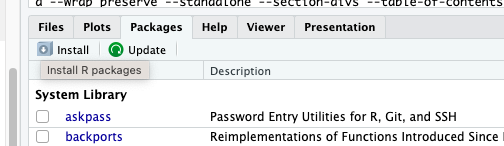
\includegraphics{images/tutorialscreenshots/installPackage.png}
  \item
    Click \textbf{Install}, type \texttt{bookdown} in the \textbf{Packages} box, and click \textbf{Install}.

    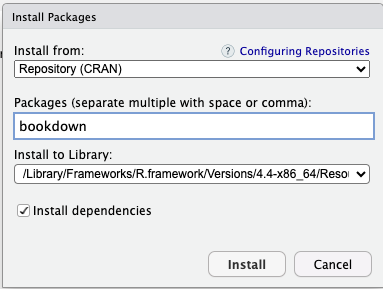
\includegraphics{images/tutorialscreenshots/installBookdownPack.png}
  \end{itemize}
\item
  \textbf{Install LaTeX distribution of your choice}:
  The distribution you choose is entirely up to you and your needs. For a list of recommended LaTeX distributions please see \ref{latex-distributions}
\end{enumerate}

Once this is complete Bookdown is now installed and you are ready to create your first Bookdown project.
5. \textbf{Create a New Bookdown Project in RStudio}:\\
- In RStudio, go to \textbf{File \textgreater{} New Project}.
- Select \textbf{New Directory} and then \textbf{Book Project using Bookdown}.
- Name your project and choose a location to save it.

\begin{enumerate}
\def\labelenumi{\arabic{enumi}.}
\setcounter{enumi}{5}
\tightlist
\item
  \textbf{Render Your Newly Created Book}:\\
  In the \textbf{Build} pane:

  \begin{itemize}
  \tightlist
  \item
    Select \textbf{Build Book} and choose your output format, or select \emph{All formats} to render your files as HTML, PDF, and EPUB.
  \item
    You can also render the book directly from the R console with the following command:
  \end{itemize}

\begin{Shaded}
\begin{Highlighting}[]
\NormalTok{bookdown}\SpecialCharTok{::}\FunctionTok{render\_book}\NormalTok{(}\StringTok{"index.Rmd"}\NormalTok{)}
\end{Highlighting}
\end{Shaded}
\end{enumerate}

\chapter{Writing and Structuring Content}\label{writing-and-structuring-content}

In this chapter, we will explore how to write and structure content in Bookdown using R Markdown syntax. Bookdown allows you to create well-organized documents by combining text, code, and references. Here, we'll cover the essentials for writing chapters, adding code chunks, creating cross-references, and structuring your content.

\section{Creating Chapters and Sections}\label{creatingchapters}

Each chapter in Bookdown is represented by a separate \texttt{.Rmd} file, and each \texttt{.Rmd} file should begin with a first-level heading, marked by a single \texttt{\#} symbol. For example:

\begin{Shaded}
\begin{Highlighting}[]
\FunctionTok{\# Chapter Title}
\end{Highlighting}
\end{Shaded}

Chapters are automatically numbered based on their order in the project directory, so make sure each file name reflects its chapter number (e.g., \texttt{02-writing-structuring-content.Rmd} for Chapter 2).

\section{Adding Sections and Subsections}\label{adding-sections-and-subsections}

You can add sections and subsections within a chapter using second-level and higher-level headings:

\begin{Shaded}
\begin{Highlighting}[]
\FunctionTok{\#\# Section Title}
\FunctionTok{\#\#\# Subsection Title}
\end{Highlighting}
\end{Shaded}

This hierarchy organizes the document according to the users needs, and these sections will automatically appear in the table of contents.

\section{Formatting Text in Bookdown}\label{formatting-text-in-bookdown}

Bookdown supports a wide range of Markdown formatting. Here are a few basics:

\begin{itemize}
\tightlist
\item
  \textbf{Bold}: \texttt{**bold\ text**} → \textbf{bold text}
\item
  \emph{Italics}: \texttt{*italicized\ text*} → \emph{italicized text}
\item
  \textbf{Bullet Points}:

  \begin{itemize}
  \tightlist
  \item
    First item
  \item
    Second item
  \end{itemize}
\item
  \textbf{Numbered Lists}:

  \begin{enumerate}
  \def\labelenumi{\arabic{enumi}.}
  \tightlist
  \item
    First item

    \begin{itemize}
    \tightlist
    \item
      Even sublists
    \item
      Like this
    \end{itemize}
  \item
    Second item
  \end{enumerate}
\end{itemize}

Use these formatting options to style text and create lists within your chapters.

\section{Adding Code Chunks}\label{adding-code-chunks}

One of the strengths of Bookdown is the ability to incorporate code into your document, whether it be R code, Markdown, LaTeX, Python, or other languages. Code chunks in R Markdown are written between three backticks (``\texttt{)\ with}\{r\}` specifying R as the language:

\begin{verbatim}

``` r
summary(cars)
```
\end{verbatim}

\subsection{Customizing Code Chunk Options}\label{customizing-code-chunk-options}

You can customize how code chunks appear using chunk options. Here are a few common options:

\begin{itemize}
\tightlist
\item
  \texttt{echo=FALSE}: Hides the code but displays the output.
\item
  \texttt{eval=FALSE}: Shows the code but does not execute it.
\item
  \texttt{fig.cap="Caption\ Text"}: Adds a caption to figures generated from the code chunk.
\item
  \texttt{out.width="50\%"}: Sets the output width for images generated in the chunk.
\end{itemize}

Example:

\begin{Shaded}
\begin{Highlighting}[]
\FunctionTok{summary}\NormalTok{(cars)}
\end{Highlighting}
\end{Shaded}

\begin{verbatim}
##      speed           dist       
##  Min.   : 4.0   Min.   :  2.00  
##  1st Qu.:12.0   1st Qu.: 26.00  
##  Median :15.0   Median : 36.00  
##  Mean   :15.4   Mean   : 42.98  
##  3rd Qu.:19.0   3rd Qu.: 56.00  
##  Max.   :25.0   Max.   :120.00
\end{verbatim}

Experiment with these options to control how your code and output appear.

\section{Cross-Referencing Sections, Figures, and Tables}\label{cross-referencing-sections-figures-and-tables}

Bookdown makes it easy to create cross-references for sections, figures, and tables.

\subsection{Cross-Referencing Sections}\label{cross-referencing-sections}

To reference a section, add an ID to the heading by including \texttt{\{\#your-id\}} at the end:

\begin{Shaded}
\begin{Highlighting}[]
\FunctionTok{\#\# Creating Chapters and Sections \{\#creatingchapters\}}
\end{Highlighting}
\end{Shaded}

Then, refer to it later in your document with:

\begin{Shaded}
\begin{Highlighting}[]
\NormalTok{See Section \textbackslash{}@ref(creatingchapters) for more information.}
\end{Highlighting}
\end{Shaded}

\subsection{Cross-Referencing Figures}\label{cross-referencing-figures}

For figures, set a chunk label and use the \texttt{fig.cap} option to add a caption:

\begin{Shaded}
\begin{Highlighting}[]
\FunctionTok{plot}\NormalTok{(cars}\SpecialCharTok{$}\NormalTok{speed, cars}\SpecialCharTok{$}\NormalTok{dist)}
\end{Highlighting}
\end{Shaded}

\begin{figure}

{\centering 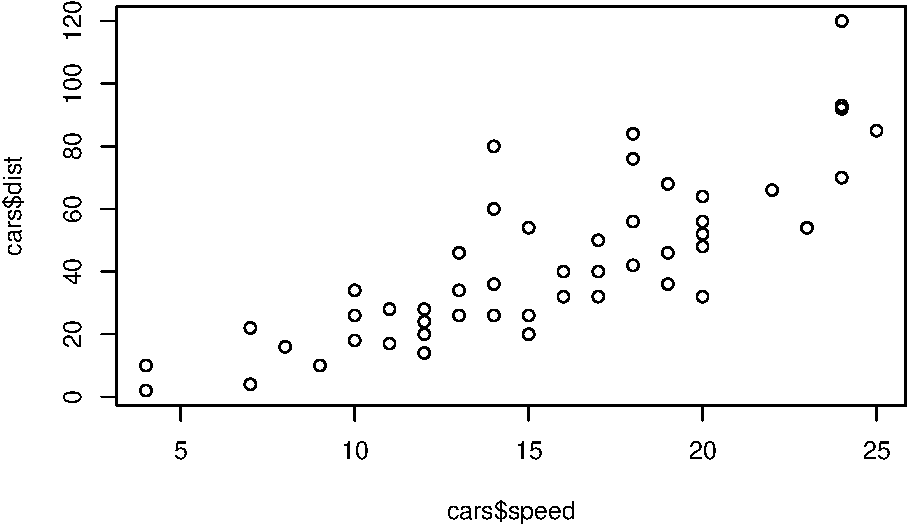
\includegraphics{_main_files/figure-latex/speed-distance-plot-1} 

}

\caption{A scatter plot of speed vs. distance}\label{fig:speed-distance-plot}
\end{figure}

You can then refer to this figure as Figure \ref{fig:speed-distance-plot}.

\subsection{Cross-Referencing Tables}\label{cross-referencing-tables}

For tables, set a chunk label. The label will automatically generate a table reference:

\begin{Shaded}
\begin{Highlighting}[]
\NormalTok{knitr}\SpecialCharTok{::}\FunctionTok{kable}\NormalTok{(}\FunctionTok{head}\NormalTok{(cars), }\AttributeTok{caption =} \StringTok{"Table of the first rows of the cars dataset"}\NormalTok{)}
\end{Highlighting}
\end{Shaded}

\begin{table}

\caption{\label{tab:cars-table}Table of the first rows of the cars dataset}
\centering
\begin{tabular}[t]{r|r}
\hline
speed & dist\\
\hline
4 & 2\\
\hline
4 & 10\\
\hline
7 & 4\\
\hline
7 & 22\\
\hline
8 & 16\\
\hline
9 & 10\\
\hline
\end{tabular}
\end{table}

You can then reference it as Table \ref{tab:cars-table}.

\chapter{Cross-references}\label{cross}

Cross-references make it easier for your readers to find and link to elements in your book. In Bookdown, you can create cross-references for chapters, sub-chapters, figures, and tables.

\section{Chapters and Sub-Chapters}\label{chapters-and-sub-chapters}

There are two steps to cross-reference any heading:

\begin{enumerate}
\def\labelenumi{\arabic{enumi}.}
\item
  \textbf{Label the heading}:\\
  Add a label by placing \texttt{\{\#your-label\}} at the end of the heading:

\begin{Shaded}
\begin{Highlighting}[]
\FunctionTok{\# Hello World \{\#nice{-}label\}}
\end{Highlighting}
\end{Shaded}

  \begin{itemize}
  \item
    If you don't add a label, Bookdown will automatically generate one based on the heading title. For example, \texttt{\#\ Hello\ World} would become \texttt{\#\ Hello\ World\ \{\#hello-world\}}.
  \item
    To label an unnumbered heading, use \texttt{\{.unnumbered\}} at the end:

\begin{Shaded}
\begin{Highlighting}[]
\FunctionTok{\# Hello World \{{-}\#nice{-}label\}}
\end{Highlighting}
\end{Shaded}
  \end{itemize}
\item
  \textbf{Reference the labeled heading}:\\
  To reference a labeled heading anywhere in the text, use \texttt{\textbackslash{}@ref(label)}. For example:

\begin{Shaded}
\begin{Highlighting}[]
\NormalTok{Please see Chapter \textbackslash{}@ref(cross) for more details.}
\end{Highlighting}
\end{Shaded}

  \begin{itemize}
  \item
    If you prefer text as the link instead of a numbered reference, you can use Markdown syntax:

\begin{Shaded}
\begin{Highlighting}[]
\CommentTok{[}\OtherTok{Click here to read about cross{-}references}\CommentTok{](\#cross)}
\end{Highlighting}
\end{Shaded}
  \end{itemize}
\end{enumerate}

\section{Captioned Figures and Tables}\label{captioned-figures-and-tables}

Figures and tables with captions can also be cross-referenced from elsewhere in your book.

\subsection{Cross-Referencing Figures}\label{cross-referencing-figures-1}

To cross-reference a figure, add a chunk label and set the \texttt{fig.cap} option for the caption. Bookdown will automatically label the figure with \texttt{fig:chunk-label}.

Example:

\begin{Shaded}
\begin{Highlighting}[]
\FunctionTok{par}\NormalTok{(}\AttributeTok{mar =} \FunctionTok{c}\NormalTok{(}\DecValTok{4}\NormalTok{, }\DecValTok{4}\NormalTok{, .}\DecValTok{1}\NormalTok{, .}\DecValTok{1}\NormalTok{))}
\FunctionTok{plot}\NormalTok{(pressure, }\AttributeTok{type =} \StringTok{\textquotesingle{}b\textquotesingle{}}\NormalTok{, }\AttributeTok{pch =} \DecValTok{19}\NormalTok{)}
\end{Highlighting}
\end{Shaded}

\begin{figure}

{\centering 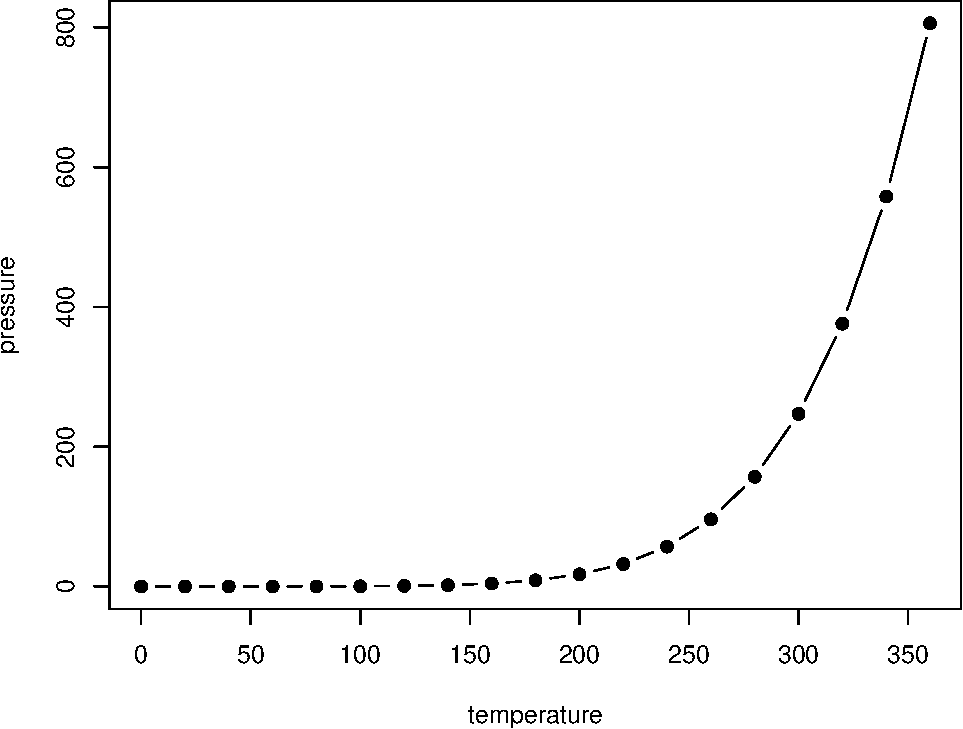
\includegraphics[width=0.8\linewidth]{_main_files/figure-latex/nice-fig-1} 

}

\caption{Here is a nice figure!}\label{fig:nice-fig}
\end{figure}

You can reference this figure using \texttt{\textbackslash{}@ref(fig:nice-fig)}. For example:

\begin{Shaded}
\begin{Highlighting}[]
\NormalTok{See Figure \textbackslash{}@ref(fig:nice{-}fig) for more details.}
\end{Highlighting}
\end{Shaded}

\subsection{Cross-Referencing Tables}\label{cross-referencing-tables-1}

To cross-reference a table, add a chunk label to the code chunk where you create the table with \texttt{knitr::kable()} and include a caption. Bookdown will automatically label the table with \texttt{tab:chunk-label}.

Example:

\begin{Shaded}
\begin{Highlighting}[]
\NormalTok{knitr}\SpecialCharTok{::}\FunctionTok{kable}\NormalTok{(}
  \FunctionTok{head}\NormalTok{(pressure, }\DecValTok{10}\NormalTok{), }\AttributeTok{caption =} \StringTok{\textquotesingle{}Here is a nice table!\textquotesingle{}}\NormalTok{,}
  \AttributeTok{booktabs =} \ConstantTok{TRUE}
\NormalTok{)}
\end{Highlighting}
\end{Shaded}

\begin{table}

\caption{\label{tab:nice-tab}Here is a nice table!}
\centering
\begin{tabular}[t]{rr}
\toprule
temperature & pressure\\
\midrule
0 & 0.0002\\
20 & 0.0012\\
40 & 0.0060\\
60 & 0.0300\\
80 & 0.0900\\
\addlinespace
100 & 0.2700\\
120 & 0.7500\\
140 & 1.8500\\
160 & 4.2000\\
180 & 8.8000\\
\bottomrule
\end{tabular}
\end{table}

You can reference this table using \texttt{\textbackslash{}@ref(tab:nice-tab)}. For example:

\begin{Shaded}
\begin{Highlighting}[]
\NormalTok{Don\textquotesingle{}t miss Table \textbackslash{}@ref(tab:nice{-}tab).}
\end{Highlighting}
\end{Shaded}

\section{Summary}\label{summary}

In this chapter, we covered how to create cross-references for headings, figures, and tables. Using cross-references helps readers navigate your document easily and allows you to create a more interactive and organized book.

Continue to the next chapter for more ways to enhance your Bookdown project.

\chapter{Customizing Output}\label{customizing-output}

In this chapter, we'll explore how to customize the output of your Bookdown project. Bookdown supports several output formats, such as HTML, PDF, and EPUB, and allows you to customize each format to match your project's needs. We'll cover choosing output formats, modifying appearance, and configuring output settings.

\section{Choosing an Output Format}\label{choosing-an-output-format}

Bookdown provides multiple output formats that allow you to publish your document in various ways:

\begin{itemize}
\tightlist
\item
  \textbf{HTML}: Ideal for online documentation or sharing on the web.
\item
  \textbf{PDF}: Useful for print-ready documents, especially for academic or professional reports.
\item
  \textbf{EPUB}: E-book format, compatible with e-readers for mobile access.
\end{itemize}

To specify output formats, edit the \texttt{\_output.yml} file in your project directory. Here's an example configuration:

\begin{Shaded}
\begin{Highlighting}[]
\AttributeTok{bookdown:}\FunctionTok{:gitbook}\KeywordTok{:}
\AttributeTok{  }\FunctionTok{css}\KeywordTok{:}\AttributeTok{ }\StringTok{"style.css"}
\AttributeTok{  }\FunctionTok{split\_by}\KeywordTok{:}\AttributeTok{ }\StringTok{"chapter"}

\AttributeTok{bookdown:}\FunctionTok{:pdf\_book}\KeywordTok{:}
\AttributeTok{  }\FunctionTok{latex\_engine}\KeywordTok{:}\AttributeTok{ xelatex}
\AttributeTok{  }\FunctionTok{citation\_package}\KeywordTok{:}\AttributeTok{ natbib}

\AttributeTok{bookdown:}\FunctionTok{:epub\_book}\KeywordTok{:}\AttributeTok{ default}
\end{Highlighting}
\end{Shaded}

This configuration tells Bookdown to create HTML (using GitBook style), PDF, and EPUB formats. Customize each format's settings to control the output style.

\section{Customizing HTML Output}\label{customizing-html-output}

To customize the HTML format, Bookdown offers the \texttt{bookdown::gitbook} and \texttt{bookdown::html\_document2} options:

\begin{itemize}
\tightlist
\item
  \textbf{GitBook}: The default HTML style, which includes a side navigation bar and a search function. This format is ideal for online documentation.
\item
  \textbf{HTML Document}: A simpler format without the sidebar, suitable for single-page reports.
\end{itemize}

You can adjust HTML settings in \texttt{\_output.yml}:

\begin{Shaded}
\begin{Highlighting}[]
\AttributeTok{bookdown:}\FunctionTok{:gitbook}\KeywordTok{:}
\AttributeTok{  }\FunctionTok{css}\KeywordTok{:}\AttributeTok{ }\StringTok{"style.css"}
\AttributeTok{  }\FunctionTok{config}\KeywordTok{:}
\AttributeTok{    }\FunctionTok{toc}\KeywordTok{:}
\AttributeTok{      }\FunctionTok{collapse}\KeywordTok{:}\AttributeTok{ section}
\AttributeTok{    }\FunctionTok{download}\KeywordTok{:}\AttributeTok{ }\KeywordTok{[}\StringTok{"pdf"}\KeywordTok{,}\AttributeTok{ }\StringTok{"epub"}\KeywordTok{]}
\end{Highlighting}
\end{Shaded}

\section{Customizing the HTML Appearance}\label{customizing-the-html-appearance}

If you want to style your HTML output further, create a \texttt{style.css} file and link it in \texttt{\_output.yml}. Here's an example of CSS customization:

\begin{Shaded}
\begin{Highlighting}[]
\CommentTok{/* style.css */}
\NormalTok{body \{}
  \KeywordTok{font{-}family}\CharTok{:} \DecValTok{Arial}\OperatorTok{,} \DecValTok{sans{-}serif}\OperatorTok{;}
\NormalTok{\}}

\NormalTok{h1}\OperatorTok{,}\NormalTok{ h2}\OperatorTok{,}\NormalTok{ h3 \{}
  \KeywordTok{color}\CharTok{:} \ConstantTok{\#2A7AE2}\OperatorTok{;}
\NormalTok{\}}

\NormalTok{code \{}
  \KeywordTok{background{-}color}\CharTok{:} \ConstantTok{\#f5f5f5}\OperatorTok{;}
  \KeywordTok{padding}\CharTok{:} \DecValTok{3}\DataTypeTok{px}\OperatorTok{;}
\NormalTok{\}}
\end{Highlighting}
\end{Shaded}

This CSS will apply a custom font, change the color of headers, and style code blocks.

\section{Customizing PDF Output}\label{customizing-pdf-output}

To generate a high-quality PDF, you'll need to install a LaTeX distribution like TinyTeX. If not already installed, you can do so in R:

\begin{Shaded}
\begin{Highlighting}[]
\FunctionTok{install.packages}\NormalTok{(}\StringTok{"tinytex"}\NormalTok{)}
\NormalTok{tinytex}\SpecialCharTok{::}\FunctionTok{install\_tinytex}\NormalTok{()}
\end{Highlighting}
\end{Shaded}

In \texttt{\_output.yml}, you can specify options to control PDF formatting:

\begin{Shaded}
\begin{Highlighting}[]
\AttributeTok{bookdown:}\FunctionTok{:pdf\_book}\KeywordTok{:}
\AttributeTok{  }\FunctionTok{latex\_engine}\KeywordTok{:}\AttributeTok{ xelatex}
\AttributeTok{  }\FunctionTok{citation\_package}\KeywordTok{:}\AttributeTok{ natbib}
\end{Highlighting}
\end{Shaded}

\begin{itemize}
\tightlist
\item
  \textbf{\texttt{latex\_engine}}: Specifies the LaTeX engine (e.g., \texttt{xelatex}, \texttt{pdflatex}). Using \texttt{xelatex} improves font compatibility.
\item
  \textbf{\texttt{citation\_package}}: Choose between \texttt{natbib} or \texttt{biblatex} for handling citations.
\end{itemize}

\section{Customizing the PDF Appearance}\label{customizing-the-pdf-appearance}

PDF customization often involves LaTeX commands. You can define appearance settings by adding a \texttt{preamble.tex} file and linking it in \texttt{\_output.yml}:

\begin{Shaded}
\begin{Highlighting}[]
\AttributeTok{bookdown:}\FunctionTok{:pdf\_book}\KeywordTok{:}
\AttributeTok{  }\FunctionTok{includes}\KeywordTok{:}
\AttributeTok{    }\FunctionTok{in\_header}\KeywordTok{:}\AttributeTok{ preamble.tex}
\end{Highlighting}
\end{Shaded}

For example, to adjust line spacing and font size in \texttt{preamble.tex}:

\begin{Shaded}
\begin{Highlighting}[]
\BuiltInTok{\textbackslash{}usepackage}\NormalTok{\{}\ExtensionTok{setspace}\NormalTok{\}}
\FunctionTok{\textbackslash{}onehalfspacing}
\BuiltInTok{\textbackslash{}usepackage}\NormalTok{\{}\ExtensionTok{geometry}\NormalTok{\}}
\FunctionTok{\textbackslash{}geometry}\NormalTok{\{margin=1in\}}
\end{Highlighting}
\end{Shaded}

This customization adjusts the line spacing to 1.5 and sets the page margins to 1 inch.

\section{Customizing EPUB Output}\label{customizing-epub-output}

To create an EPUB e-book, use \texttt{bookdown::epub\_book} in \texttt{\_output.yml}. Bookdown handles most EPUB formatting automatically, but you can make some modifications:

\begin{Shaded}
\begin{Highlighting}[]
\AttributeTok{bookdown:}\FunctionTok{:epub\_book}\KeywordTok{:}
\AttributeTok{  }\FunctionTok{stylesheet}\KeywordTok{:}\AttributeTok{ }\StringTok{"style.css"}
\AttributeTok{  }\FunctionTok{cover\_image}\KeywordTok{:}\AttributeTok{ }\StringTok{"images/cover.jpg"}
\AttributeTok{  }\FunctionTok{toc}\KeywordTok{:}\AttributeTok{ }\CharTok{yes}
\end{Highlighting}
\end{Shaded}

This configuration adds a cover image, applies the CSS stylesheet, and includes a table of contents.

\section{\texorpdfstring{Specifying Global Settings in \texttt{\_bookdown.yml}}{Specifying Global Settings in \_bookdown.yml}}\label{specifying-global-settings-in-_bookdown.yml}

The \texttt{\_bookdown.yml} file allows you to set global configurations, such as the order of chapters, the naming convention for output files, and the label format for figures and tables. Here's an example:

\begin{Shaded}
\begin{Highlighting}[]
\FunctionTok{book\_filename}\KeywordTok{:}\AttributeTok{ }\StringTok{"my{-}book"}
\FunctionTok{rmd\_files}\KeywordTok{:}\AttributeTok{ }\KeywordTok{[}\StringTok{"index.Rmd"}\KeywordTok{,}\AttributeTok{ }\StringTok{"01{-}introduction.Rmd"}\KeywordTok{,}\AttributeTok{ }\StringTok{"02{-}writing{-}structuring{-}content.Rmd"}\KeywordTok{,}\AttributeTok{ }\StringTok{"03{-}customizing{-}output.Rmd"}\KeywordTok{]}
\FunctionTok{language}\KeywordTok{:}
\AttributeTok{  }\FunctionTok{label}\KeywordTok{:}
\AttributeTok{    }\FunctionTok{fig}\KeywordTok{:}\AttributeTok{ }\StringTok{"Figure "}
\AttributeTok{    }\FunctionTok{tab}\KeywordTok{:}\AttributeTok{ }\StringTok{"Table "}
\FunctionTok{delete\_merged\_file}\KeywordTok{:}\AttributeTok{ }\CharTok{true}
\end{Highlighting}
\end{Shaded}

\begin{itemize}
\tightlist
\item
  \textbf{\texttt{book\_filename}}: Sets the base filename for output files.
\item
  \textbf{\texttt{rmd\_files}}: Specifies the order of chapters.
\item
  \textbf{\texttt{language.label}}: Customizes labels for figures and tables.
\item
  \textbf{\texttt{delete\_merged\_file}}: Deletes intermediary files after rendering, keeping the directory clean.
\end{itemize}

\section{Example Output}\label{example-output}

To render all formats simultaneously, you can use the \texttt{render\_book()} function in the R console:

\begin{Shaded}
\begin{Highlighting}[]
\NormalTok{bookdown}\SpecialCharTok{::}\FunctionTok{render\_book}\NormalTok{(}\StringTok{"index.Rmd"}\NormalTok{, }\AttributeTok{output\_format =} \StringTok{"all"}\NormalTok{)}
\end{Highlighting}
\end{Shaded}

This command generates HTML, PDF, and EPUB files as specified in \texttt{\_output.yml}.

\chapter{Advanced Features and Practical Example}\label{advanced-features-and-practical-example}

In this chapter, we'll explore some advanced features of Bookdown, including adding citations, managing bibliographies, and using practical examples to illustrate how to apply these features in real projects.

\section{Adding Citations and Managing References}\label{adding-citations-and-managing-references}

Bookdown makes it easy to manage references and add citations by using BibTeX files. Here's how to set up and include references in your Bookdown project.

\subsection{\texorpdfstring{Step 1: Create a \texttt{.bib} File}{Step 1: Create a .bib File}}\label{step-1-create-a-.bib-file}

First, create a \texttt{.bib} file for your references (e.g., \texttt{references.bib}). You can add references in BibTeX format. Here's an example entry:

\begin{Shaded}
\begin{Highlighting}[]
\VariableTok{@article}\NormalTok{\{}\OtherTok{abatzoglou2016}\NormalTok{,}
  \DataTypeTok{title}\NormalTok{     = \{Impact of anthropogenic climate change on wildfire across western US forests\},}
  \DataTypeTok{author}\NormalTok{    = \{Abatzoglou, J. T. and Williams, A. P.\},}
  \DataTypeTok{year}\NormalTok{      = \{2016\},}
  \DataTypeTok{journal}\NormalTok{   = \{Proceedings of the National Academy of Sciences\},}
  \DataTypeTok{volume}\NormalTok{    = \{113\},}
  \DataTypeTok{number}\NormalTok{    = \{42\},}
  \DataTypeTok{pages}\NormalTok{     = \{11770{-}{-}11775\},}
  \DataTypeTok{doi}\NormalTok{       = \{10.1073/pnas.1607171113\}}
\NormalTok{\}}
\end{Highlighting}
\end{Shaded}

\subsection{\texorpdfstring{Step 2: Link the \texttt{.bib} File in \texttt{index.Rmd}}{Step 2: Link the .bib File in index.Rmd}}\label{step-2-link-the-.bib-file-in-index.rmd}

In your \texttt{index.Rmd} file, include the \texttt{.bib} file in the YAML header:

\begin{Shaded}
\begin{Highlighting}[]
\FunctionTok{bibliography}\KeywordTok{:}\AttributeTok{ }\KeywordTok{[}\AttributeTok{references.bib}\KeywordTok{]}
\FunctionTok{link{-}citations}\KeywordTok{:}\AttributeTok{ }\CharTok{yes}
\end{Highlighting}
\end{Shaded}

\subsection{Step 3: Cite Sources in Your Text}\label{step-3-cite-sources-in-your-text}

To cite a source, use \texttt{{[}@citation-key{]}} in your text, where \texttt{citation-key} matches the key in your \texttt{.bib} file (e.g., \texttt{{[}@abatzoglou2016{]}}). For example:

\begin{Shaded}
\begin{Highlighting}[]
\NormalTok{Studies have shown the impact of climate change on wildfire intensity in western US forests }\CommentTok{[}\OtherTok{@abatzoglou2016}\CommentTok{]}\NormalTok{.}
\end{Highlighting}
\end{Shaded}

Bookdown will automatically format your citation based on the output style.

\subsection{Step 4: Customize Citation Style (Optional)}\label{step-4-customize-citation-style-optional}

If you need a specific citation style, you can add a \texttt{.csl} (Citation Style Language) file in your project and reference it in the YAML header:

\begin{Shaded}
\begin{Highlighting}[]
\FunctionTok{csl}\KeywordTok{:}\AttributeTok{ }\StringTok{"chicago{-}author{-}date.csl"}
\end{Highlighting}
\end{Shaded}

Download \texttt{.csl} files from sources like \href{https://www.zotero.org/styles}{Zotero}.

\section{Using Cross-References with Citations}\label{using-cross-references-with-citations}

In addition to referencing external sources, Bookdown allows you to cross-reference sections, figures, and tables, as discussed in Chapter 2. For example:

\begin{Shaded}
\begin{Highlighting}[]
\NormalTok{As shown in Figure \textbackslash{}@ref(fig:example{-}figure), the trend is evident.}
\end{Highlighting}
\end{Shaded}

Using cross-references with citations helps keep your document organized and easy to navigate.

\section{Practical Example: Incorporating an Existing Paper}\label{practical-example-incorporating-an-existing-paper}

Let's walk through using Bookdown to incorporate an existing paper or document as part of your Bookdown project. This example will cover integrating content, images, and citations.

\subsection{Step 1: Import the Document Content}\label{step-1-import-the-document-content}

To add an existing document, start by copying sections of the text into a new \texttt{.Rmd} file, such as \texttt{05-existing-paper.Rmd}. Organize it with headings and sections as needed:

\begin{Shaded}
\begin{Highlighting}[]
\FunctionTok{\# Example Paper: Drought in California}

\FunctionTok{\#\# Introduction}

\NormalTok{Droughts are a recurring issue in California, impacting water availability, agriculture, and the environment. Research has shown that climate change exacerbates the frequency and severity of drought events }\CommentTok{[}\OtherTok{@abatzoglou2016}\CommentTok{]}\NormalTok{.}

\FunctionTok{\#\# Causes of Drought}

\NormalTok{Several factors contribute to drought conditions, including atmospheric patterns, precipitation deficits, and temperature increases.}

\FunctionTok{\#\# Socioeconomic Impacts}

\NormalTok{The economic impact of droughts can be severe, particularly in agriculture{-}dependent regions.}
\end{Highlighting}
\end{Shaded}

\subsection{Step 2: Add Figures and Tables}\label{step-2-add-figures-and-tables}

If your paper includes figures and tables, add them as code chunks or external images using \texttt{knitr::include\_graphics()} for images:

\begin{figure}
\centering
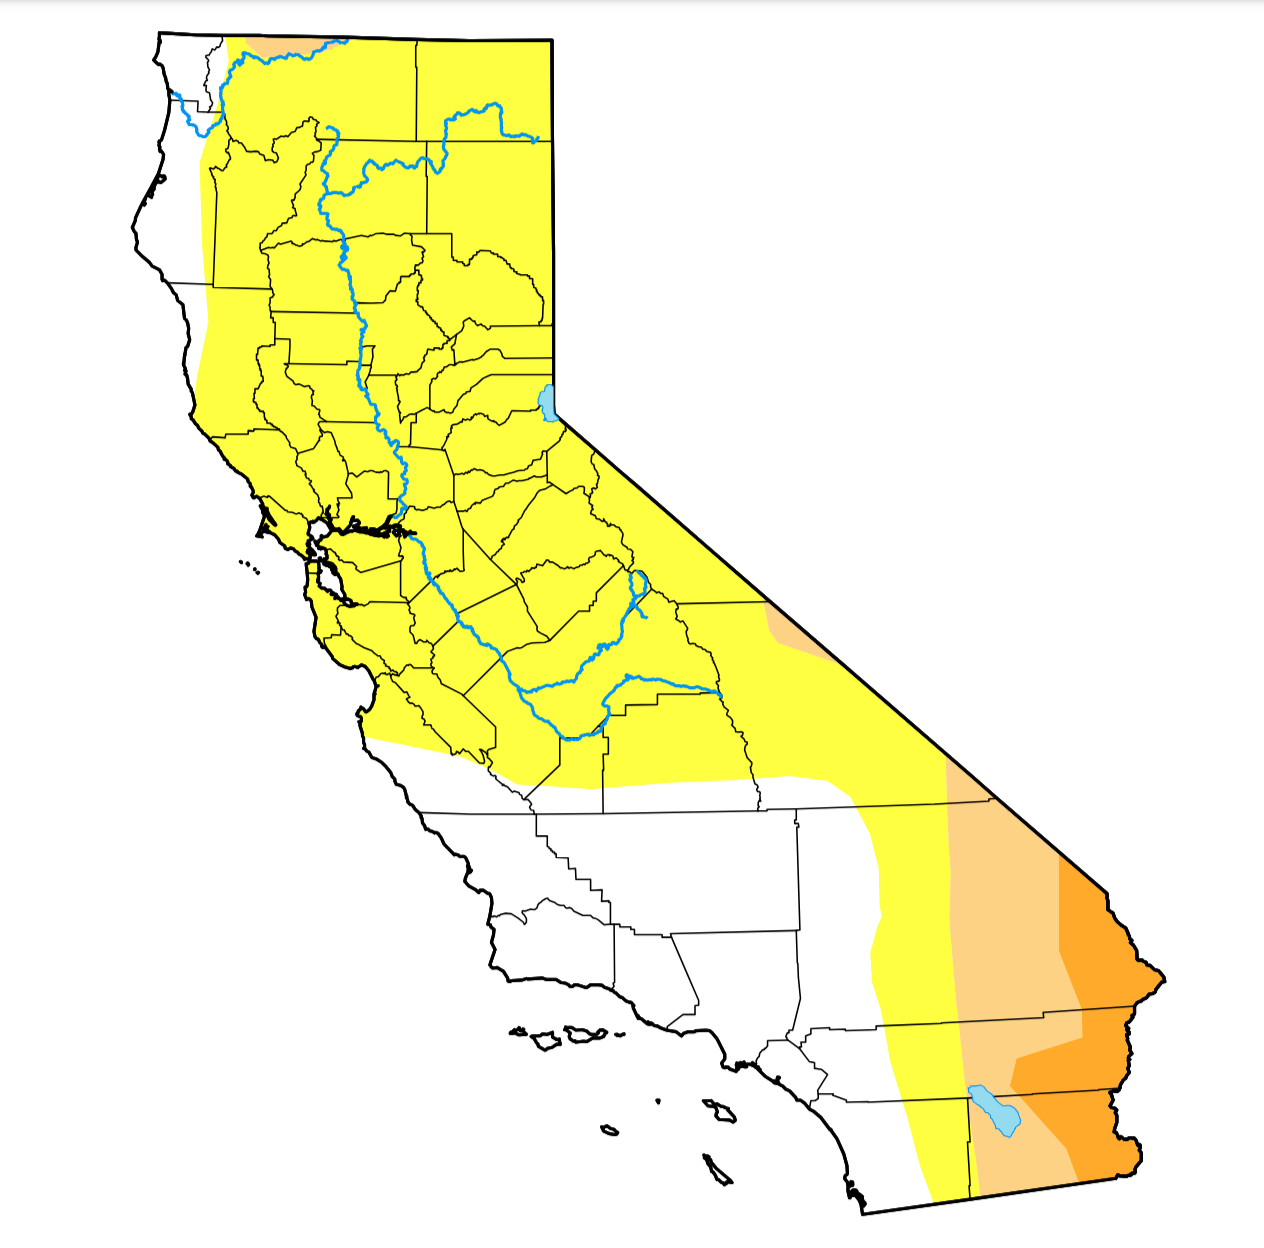
\includegraphics{images/drought-map.png}
\caption{\label{fig:unnamed-chunk-7}Example of a drought map in California}
\end{figure}

For tables, use \texttt{knitr::kable()} to format data as a table:

\begin{verbatim}

``` r
knitr::kable(head(drought_data), caption = "Drought data for California")
```
\end{verbatim}

\subsection{Step 3: Integrate Citations}\label{step-3-integrate-citations}

If the paper includes citations, ensure each citation is included in your \texttt{.bib} file and cite them using the \texttt{{[}@citation-key{]}} format as needed. For example:

\begin{Shaded}
\begin{Highlighting}[]
\NormalTok{The effects of droughts on ecosystems have been widely studied }\CommentTok{[}\OtherTok{@pompeii2020}\CommentTok{]}\NormalTok{.}
\end{Highlighting}
\end{Shaded}

\subsection{Step 4: Create a Table of Contents and Links}\label{step-4-create-a-table-of-contents-and-links}

As your document grows, Bookdown will automatically create a table of contents for easy navigation. Use cross-references to link sections, figures, and tables within the text. For example:

\begin{Shaded}
\begin{Highlighting}[]
\NormalTok{As discussed in Section \textbackslash{}@ref(causes{-}drought), various factors contribute to drought conditions.}
\end{Highlighting}
\end{Shaded}

This will create a clickable link in HTML output, making it easier for readers to navigate.

\section{Example Output and Render Settings}\label{example-output-and-render-settings}

To render the final output with all citations, cross-references, and figures, make sure the YAML header in \texttt{\_output.yml} specifies the output formats you need (HTML, PDF, or EPUB). Use the following command in the R console to render all formats:

\begin{verbatim}
bookdown::render_book("index.Rmd", output_format = "all")
\end{verbatim}

\section{Conclusion}\label{conclusion}

In this chapter, you've learned how to use advanced Bookdown features like citations, cross-references, and practical examples. By integrating an existing paper, you've seen how Bookdown can bring together complex content with ease. You now have the tools to create a comprehensive, structured document with citations, images, tables, and references.

With these skills, you're ready to produce high-quality documentation for academic, professional, or personal projects.

\chapter{Blocks}\label{blocks}

\section{Equations}\label{equations}

Here is an equation.

\begin{equation} 
  f\left(k\right) = \binom{n}{k} p^k\left(1-p\right)^{n-k}
  \label{eq:binom}
\end{equation}

You may refer to using \texttt{\textbackslash{}@ref(eq:binom)}, like see Equation \eqref{eq:binom}.

\section{Theorems and proofs}\label{theorems-and-proofs}

Labeled theorems can be referenced in text using \texttt{\textbackslash{}@ref(thm:tri)}, for example, check out this smart theorem \ref{thm:tri}.

\begin{theorem}
\protect\hypertarget{thm:tri}{}\label{thm:tri}For a right triangle, if \(c\) denotes the \emph{length} of the hypotenuse
and \(a\) and \(b\) denote the lengths of the \textbf{other} two sides, we have
\[a^2 + b^2 = c^2\]
\end{theorem}

Read more here \url{https://bookdown.org/yihui/bookdown/markdown-extensions-by-bookdown.html}.

\section{Callout blocks}\label{callout-blocks}

The R Markdown Cookbook provides more help on how to use custom blocks to design your own callouts: \url{https://bookdown.org/yihui/rmarkdown-cookbook/custom-blocks.html}

\chapter{Sharing your book}\label{sharing-your-book}

\section{Publishing}\label{publishing}

HTML books can be published online, see: \url{https://bookdown.org/yihui/bookdown/publishing.html}

\section{404 pages}\label{pages}

By default, users will be directed to a 404 page if they try to access a webpage that cannot be found. If you'd like to customize your 404 page instead of using the default, you may add either a \texttt{\_404.Rmd} or \texttt{\_404.md} file to your project root and use code and/or Markdown syntax.

\section{Metadata for sharing}\label{metadata-for-sharing}

Bookdown HTML books will provide HTML metadata for social sharing on platforms like Twitter, Facebook, and LinkedIn, using information you provide in the \texttt{index.Rmd} YAML. To setup, set the \texttt{url} for your book and the path to your \texttt{cover-image} file. Your book's \texttt{title} and \texttt{description} are also used.

This \texttt{gitbook} uses the same social sharing data across all chapters in your book- all links shared will look the same.

Specify your book's source repository on GitHub using the \texttt{edit} key under the configuration options in the \texttt{\_output.yml} file, which allows users to suggest an edit by linking to a chapter's source file.

Read more about the features of this output format here:

\url{https://pkgs.rstudio.com/bookdown/reference/gitbook.html}

Or use:

\begin{Shaded}
\begin{Highlighting}[]
\NormalTok{?bookdown}\SpecialCharTok{::}\NormalTok{gitbook}
\end{Highlighting}
\end{Shaded}

\chapter{LaTeX Distributions for Bookdown}\label{latex-distributions-for-bookdown}

To render PDF outputs with Bookdown, you need to install a LaTeX distribution. Below is a list of popular options, categorized by operating system and user preferences:

\section{Recommended LaTeX Distributions}\label{recommended-latex-distributions}

\subsection{\texorpdfstring{1. \textbf{TinyTeX} (Recommended)}{1. TinyTeX (Recommended)}}\label{tinytex-recommended}

\begin{itemize}
\item
  \textbf{Description}: A lightweight, cross-platform LaTeX distribution designed to work seamlessly with R and Bookdown.
\item
  \textbf{Installation}: Run the following commands in R:

\begin{Shaded}
\begin{Highlighting}[]
\FunctionTok{install.packages}\NormalTok{(}\StringTok{"tinytex"}\NormalTok{)}
\NormalTok{tinytex}\SpecialCharTok{::}\FunctionTok{install\_tinytex}\NormalTok{()}
\end{Highlighting}
\end{Shaded}
\item
  \textbf{Advantages}:

  \begin{itemize}
  \tightlist
  \item
    Minimal installation size.
  \item
    Automatically installs missing packages when rendering.
  \end{itemize}
\item
  \textbf{Website}: \href{https://yihui.org/tinytex/}{TinyTeX Documentation}
\end{itemize}

\begin{center}\rule{0.5\linewidth}{0.5pt}\end{center}

\section{Additional LaTeX Distributions}\label{additional-latex-distributions}

\subsection{\texorpdfstring{2. \textbf{TeX Live}}{2. TeX Live}}\label{tex-live}

\begin{itemize}
\tightlist
\item
  \textbf{Description}: A comprehensive LaTeX distribution suitable for Linux and cross-platform users.
\item
  \textbf{Installation}:

  \begin{itemize}
  \item
    \textbf{Linux}:

\begin{Shaded}
\begin{Highlighting}[]
\FunctionTok{sudo}\NormalTok{ apt{-}get install texlive{-}full}
\end{Highlighting}
\end{Shaded}
  \item
    \textbf{macOS and Windows}: Download from \href{https://www.tug.org/texlive/}{TeX Live}.
  \end{itemize}
\item
  \textbf{Advantages}:

  \begin{itemize}
  \tightlist
  \item
    Full-featured with a vast collection of LaTeX packages.
  \item
    Stable and widely used.
  \end{itemize}
\item
  \textbf{Website}: \href{https://www.tug.org/texlive/}{TeX Live Documentation}
\end{itemize}

\begin{center}\rule{0.5\linewidth}{0.5pt}\end{center}

\subsection{\texorpdfstring{3. \textbf{MikTeX}}{3. MikTeX}}\label{miktex}

\begin{itemize}
\tightlist
\item
  \textbf{Description}: A user-friendly LaTeX distribution popular among Windows users.
\item
  \textbf{Installation}: Download and install from \href{https://miktex.org/}{MikTeX}.
\item
  \textbf{Advantages}:

  \begin{itemize}
  \tightlist
  \item
    On-demand installation of missing packages.
  \item
    Easy-to-use package manager.
  \end{itemize}
\item
  \textbf{Website}: \href{https://miktex.org/}{MikTeX Documentation}
\end{itemize}

\begin{center}\rule{0.5\linewidth}{0.5pt}\end{center}

\subsection{\texorpdfstring{4. \textbf{MacTeX} (for macOS)}{4. MacTeX (for macOS)}}\label{mactex-for-macos}

\begin{itemize}
\tightlist
\item
  \textbf{Description}: A macOS-specific version of TeX Live with additional tools for macOS users.
\item
  \textbf{Installation}: Download and install from \href{https://www.tug.org/mactex/}{MacTeX}.
\item
  \textbf{Advantages}:

  \begin{itemize}
  \tightlist
  \item
    Tailored for macOS with GUI tools like TeXShop.
  \item
    Includes a full TeX Live distribution.
  \end{itemize}
\item
  \textbf{Website}: \href{https://www.tug.org/mactex/}{MacTeX Documentation}
\end{itemize}

\begin{center}\rule{0.5\linewidth}{0.5pt}\end{center}

\subsection{\texorpdfstring{5. \textbf{ProTeXt} (for Windows)}{5. ProTeXt (for Windows)}}\label{protext-for-windows}

\begin{itemize}
\tightlist
\item
  \textbf{Description}: A Windows-specific distribution that combines MikTeX with a user-friendly installer.
\item
  \textbf{Installation}: Download and install from \href{https://www.tug.org/protext/}{ProTeXt}.
\item
  \textbf{Advantages}:

  \begin{itemize}
  \tightlist
  \item
    Streamlined setup for beginners.
  \item
    Integrates LaTeX editors like TeXworks.
  \end{itemize}
\item
  \textbf{Website}: \href{https://www.tug.org/protext/}{ProTeXt Documentation}
\end{itemize}

\begin{center}\rule{0.5\linewidth}{0.5pt}\end{center}

Choose the distribution that best fits your operating system and needs. For most users, TinyTeX is the easiest to install and manage, especially if you're using R and Bookdown.

\chapter{Drought in California}\label{drought-in-california}

\section{Introduction}\label{introduction}

Droughts in California are a critical environmental issue that affects the state's water availability, agricultural sectors, and overall economy. California is known for its agricultural products and growing population, but it is also known for frequent droughts that have severely impacted the state's water resources. With the effects of climate change continuing to alter global weather patterns, droughts in the state are becoming more frequent and intense. These changes not only threaten the stability of California's agriculture but also jeopardize the water supply for millions of residents, leading to severe economic and environmental consequences. Additionally, droughts increase the risk of wildfires, which can cause widespread destruction and further strain water resources. In order to better understand drought in California, this chapter will explore the phenomenon of drought by focusing on its causes, socioeconomic impacts, effects on wildfires, the links between climate change and drought, and potential mitigation strategies.

\section{Types of Droughts}\label{types-of-droughts}

Droughts occur when there is a prolonged period of inadequate rainfall, resulting in a water shortage that impacts agricultural water supplies, municipal water systems, and natural ecosystems. Several types of droughts affect different aspects of the environment and society:

\begin{itemize}
\tightlist
\item
  \textbf{Meteorological drought}: A deficiency in precipitation over a specific period, often measured against long-term regional averages, and typically the first indicator of drought conditions.
\item
  \textbf{Agricultural drought}: Occurs when insufficient soil moisture affects crop growth and yields, threatening food production and farming livelihoods.
\item
  \textbf{Hydrological drought}: Involves the depletion of water resources in rivers, lakes, reservoirs, and groundwater systems, often following extended meteorological drought periods, with significant consequences for irrigation, drinking water supplies, and industrial uses.
\item
  \textbf{Socioeconomic drought}: Arises when the demand for water exceeds the available supply, leading to economic disruptions, particularly in water-dependent sectors like agriculture and energy.
\item
  \textbf{Ecological drought}: Impacts ecosystem health, resulting in biodiversity loss, habitat disruption, and changes in ecosystem functions due to prolonged water shortages.
\end{itemize}

In recent years, flash droughts, where conditions rapidly worsen due to rising temperatures, have become more frequent as a result of global climate change \citep{walker2023}.

\section{Causes of Drought in California}\label{causes-of-drought-in-california}

The causes of drought in California are multifaceted, involving both natural and anthropogenic factors. One primary natural cause is Pacific Sea surface temperature anomalies, which lead to persistent high-pressure systems that block rainstorms from reaching the state. This phenomenon disrupts atmospheric circulation and reduces precipitation across California, creating prolonged dry periods \citep{wei2016}. However, human-induced climate change has also significantly contributed to the severity of these droughts. Between 2012 and 2014, anthropogenic warming was estimated to account for 8-27\% of the drought conditions experienced in California, exacerbating the natural variability of drought patterns in the region \citep{williams2015}. This combination of natural variability and human-induced changes has not only increased the frequency, length, and intensity of droughts but has also strained the state's water infrastructure.

\section{Socioeconomic Impacts}\label{socioeconomic-impacts}

The socio-economic impacts of drought in California are profound. California's agricultural industry is highly dependent on easily available water, but during periods of drought, it suffers significant losses. For instance, the 2015 drought led to a reduction of 2.6 million acre-feet in water supply and an economic loss of \$1.8 billion. This caused approximately 564,000 acres of farmland to be fallowed, directly impacting agricultural revenues and employment \citep{sumner2015}. The drought also highlighted inequalities in water access, with rural communities in agricultural regions, such as Tulare County, being disproportionately affected. These communities experienced domestic well failures, emphasizing the social aspect of water scarcity in the state \citep{pompeii2020}. Environmental impacts are another significant concern, as droughts increase wildfire risks and degrade ecosystems dependent on adequate water supplies. Reduced water levels in rivers, lakes, and reservoirs also threaten fish and aquatic populations, leading to long-term ecological consequences.

\section{Wildfire Risk}\label{wildfire-risk}

One of the most significant effects of prolonged drought in California is the increased frequency and intensity of wildfires. Droughts create dry conditions, causing vegetation like grasses and trees to lose moisture and become more flammable. Without adequate rainfall, even typically fire-resistant plants dry out, providing fuel for wildfires. According to \citet{westerling2019}, a significant portion of forest fires in the western United States can be linked to drought, which has extended fire seasons and increased the areas burned. Drought-induced wildfires have devastating effects on both the environment and human communities. They destroy homes, displace residents, and damage ecosystems while also leading to carbon emissions from burning vegetation \citep{abatzoglou2016}.

\section{Climate Change and Drought}\label{climate-change-and-drought}

Climate change is a major driver of the increasing frequency and severity of droughts in California. As global temperatures continue to rise, so do evaporation rates, which reduces available surface water and soil moisture. This exacerbates the conditions that cause droughts, worsening their impacts on agriculture, water resources, and ecosystems. The 2013-2014 drought in California was partially attributed to climate change, which intensified the effects of naturally occurring weather patterns, like high-pressure systems that block rainfall \citep{mao2015}.

\section{Mitigation Strategies}\label{mitigation-strategies}

California has implemented a range of strategies to mitigate the impacts of drought, focusing on both immediate responses and long-term solutions. Water conservation, wastewater recycling, and water transfers are among the most commonly used methods. Conservation efforts, such as public water-use restrictions and the promotion of water-efficient technologies in households and agriculture, play a significant role in reducing water demand during drought periods. Wastewater recycling, in particular, has been gaining traction as a long-term solution, although it continues to face political and public resistance \citep{keavney2022}. Water transfers, which involve reallocating water from one region to another, provide flexibility in water management, helping to address shortages where they are most acute. Replenishing groundwater aquifers is another critical strategy, as aquifer depletion during droughts can lead to long-term water scarcity. Managed aquifer recharge (MAR) initiatives, which involve intentionally refilling underground aquifers during wet periods, are increasingly recognized as a sustainable way to bolster water supplies for future droughts. During the 2012-2016 drought, ranchers in California adapted by employing more proactive drought management practices, such as drip irrigation and efficient water delivery systems, which were shaped by their past experiences with severe droughts \citep{woodmansee2021}.

\section{Conclusion}\label{conclusion-1}

Drought in California represents a vast and complex challenge that affects all aspects of life in the state, from agriculture to urban water supplies. The causes of drought are both natural and human-induced, showing a need for a comprehensive approach in addressing it. Climate change continues to play a critical role in exacerbating drought conditions, while the socio-economic impacts of drought are severe, particularly in rural agricultural communities and ecosystems that depend on reliable water supplies. Moving forward, a combination of policy reform, technological innovation, public engagement, and enhanced infrastructure for groundwater replenishment and water recycling will be crucial in addressing California's long-term water challenges.

\chapter{LaTeX in Bookdown}\label{latex-in-bookdown}

Bookdown offers powerful support for LaTeX, allowing you to seamlessly integrate any LaTeX packages you need into your documents. Whether you're working with mathematical equations, theorems, lemmas, proofs, or other advanced features, this tutorial will guide you through the essentials of using LaTeX in Bookdown, showing you how to effectively incorporate and reference these elements.

\begin{center}\rule{0.5\linewidth}{0.5pt}\end{center}

\section{Including LaTeX Packages in Bookdown}\label{including-latex-packages-in-bookdown}

One of the powerful features of Bookdown is its seamless integration with LaTeX, allowing you to include any LaTeX package that suits your needs. This flexibility is especially useful when working with advanced mathematical notations, custom formatting, or specialized content.

\subsection{\texorpdfstring{Using a \texttt{preamble.tex} File}{Using a preamble.tex File}}\label{using-a-preamble.tex-file}

To include LaTeX packages, you can create a \texttt{preamble.tex} file and link it in your \texttt{\_output.yml} file. The \texttt{preamble.tex} file is processed before the document is rendered, making it the ideal place to load additional LaTeX packages.

\begin{enumerate}
\def\labelenumi{\arabic{enumi}.}
\item
  \textbf{Create a \texttt{preamble.tex} File}\\
  Add any LaTeX package you want to use in your document. For example here is a list of packages that are typically used by students first introduced to LaTeX:

\begin{Shaded}
\begin{Highlighting}[]
\CommentTok{\% preamble.tex}
\BuiltInTok{\textbackslash{}usepackage}\NormalTok{\{}\ExtensionTok{booktabs}\NormalTok{\}}
\BuiltInTok{\textbackslash{}usepackage}\NormalTok{\{}\ExtensionTok{amssymb}\NormalTok{\}}
\BuiltInTok{\textbackslash{}usepackage}\NormalTok{\{}\ExtensionTok{amsmath}\NormalTok{\}}
\BuiltInTok{\textbackslash{}usepackage}\NormalTok{\{}\ExtensionTok{graphicx}\NormalTok{\}}
\BuiltInTok{\textbackslash{}usepackage}\NormalTok{\{}\ExtensionTok{wasysym}\NormalTok{\}}
\BuiltInTok{\textbackslash{}usepackage}\NormalTok{\{}\ExtensionTok{amsthm}\NormalTok{\}}
\BuiltInTok{\textbackslash{}usepackage}\NormalTok{\{}\ExtensionTok{multirow}\NormalTok{\}}
\BuiltInTok{\textbackslash{}usepackage}\NormalTok{\{}\ExtensionTok{epsf}\NormalTok{\}}
\BuiltInTok{\textbackslash{}usepackage}\NormalTok{\{}\ExtensionTok{tikz}\NormalTok{\}}
\BuiltInTok{\textbackslash{}usepackage}\NormalTok{\{}\ExtensionTok{cancel}\NormalTok{\}}
\BuiltInTok{\textbackslash{}usepackage}\NormalTok{\{}\ExtensionTok{hyperref}\NormalTok{\}}
\BuiltInTok{\textbackslash{}usepackage}\NormalTok{\{}\ExtensionTok{gensymb}\NormalTok{\}}
\BuiltInTok{\textbackslash{}usepackage}\NormalTok{\{}\ExtensionTok{marvosym}\NormalTok{\}}
\end{Highlighting}
\end{Shaded}
\item
  \textbf{Link \texttt{preamble.tex} in \texttt{\_output.yml}}\\
  Update your \texttt{\_output.yml} file to include the \texttt{preamble.tex} file for PDF output:

\begin{Shaded}
\begin{Highlighting}[]
\AttributeTok{bookdown:}\FunctionTok{:pdf\_book}\KeywordTok{:}
\AttributeTok{  }\FunctionTok{latex\_engine}\KeywordTok{:}\AttributeTok{ xelatex}
\AttributeTok{  }\FunctionTok{includes}\KeywordTok{:}
\AttributeTok{    }\FunctionTok{in\_header}\KeywordTok{:}\AttributeTok{ preamble.tex}
\end{Highlighting}
\end{Shaded}
\end{enumerate}

\subsection{Example: Using AMSMath}\label{example-using-amsmath}

Once the \texttt{amsmath} package is included, you can use its features, such as environments for aligned equations:

\begin{Shaded}
\begin{Highlighting}[]
\NormalTok{\textbackslash{}begin\{align\}}
\NormalTok{  a + b \&= c }\SpecialCharTok{\textbackslash{}\textbackslash{}}
\NormalTok{  x {-} y \&= z}
\NormalTok{\textbackslash{}end\{align\}}
\end{Highlighting}
\end{Shaded}

\subsection{Adding Multiple Packages}\label{adding-multiple-packages}

You can include as many packages as you need in the \texttt{preamble.tex} file. For example:

\begin{Shaded}
\begin{Highlighting}[]
\CommentTok{\% preamble.tex}
\BuiltInTok{\textbackslash{}usepackage}\NormalTok{\{}\ExtensionTok{amsmath, amssymb}\NormalTok{\} }\CommentTok{\% Math packages}
\BuiltInTok{\textbackslash{}usepackage}\NormalTok{\{}\ExtensionTok{color}\NormalTok{\} }\CommentTok{\% For colored text}
\BuiltInTok{\textbackslash{}usepackage}\NormalTok{\{}\ExtensionTok{hyperref}\NormalTok{\} }\CommentTok{\% For hyperlinks}
\BuiltInTok{\textbackslash{}usepackage}\NormalTok{\{}\ExtensionTok{booktabs}\NormalTok{\} }\CommentTok{\% For enhanced table formatting}
\end{Highlighting}
\end{Shaded}

\subsection{Tips for Using LaTeX Packages}\label{tips-for-using-latex-packages}

\begin{enumerate}
\def\labelenumi{\arabic{enumi}.}
\item
  \textbf{Ensure Compatibility}: Some LaTeX packages may conflict with each other. If errors occur, review the documentation for each package to ensure compatibility.
\item
  \textbf{Use the Right LaTeX Engine}: Some packages (e.g., those using custom fonts) may require a specific LaTeX engine, such as \texttt{xelatex} or \texttt{lualatex}. Specify the engine in \texttt{\_output.yml}:

\begin{Shaded}
\begin{Highlighting}[]
\AttributeTok{bookdown:}\FunctionTok{:pdf\_book}\KeywordTok{:}
\AttributeTok{  }\FunctionTok{latex\_engine}\KeywordTok{:}\AttributeTok{ xelatex}
\end{Highlighting}
\end{Shaded}
\item
  \textbf{Debugging Errors}: If your document fails to compile, check the error message in the console or look at the \texttt{.log} file generated by LaTeX for troubleshooting.
\end{enumerate}

By including custom LaTeX packages, you can extend the functionality of your Bookdown project to suit your unique requirements, whether it's for academic papers, technical documents, or books.

\section{Mathematical Equations}\label{mathematical-equations}

LaTeX is widely used for formatting mathematical equations. Bookdown makes it easy to include both inline and display-style equations.

\subsection{Inline Equations}\label{inline-equations}

Use \texttt{\$...\$} to include inline math equations within your text. The following code:

\begin{Shaded}
\begin{Highlighting}[]
\NormalTok{The formula for the area of a circle is $( A = \textbackslash{}pi r\^{}2 )$, where $( r )$ is the radius.}
\end{Highlighting}
\end{Shaded}

Is then displayed as follows:

The formula for the area of a circle is \(( A = \pi r^2 )\), where \(( r )\) is the radius.

\subsection{Display Equations}\label{display-equations}

For equations that you may want to have on their own line you have two options. You can surround your LaTeX code \texttt{\$\$...\$\$} or alternatively use the LaTeX \texttt{equation} environment.

Here we see the usage of \texttt{\$\$...\$\$}

\begin{Shaded}
\begin{Highlighting}[]
\NormalTok{$$}
\NormalTok{E = mc\^{}2}
\NormalTok{$$}
\end{Highlighting}
\end{Shaded}

Which gives us:

\[
E = mc^2
\]

Here we are using the \texttt{equation} environment with a label:

\begin{Shaded}
\begin{Highlighting}[]

\NormalTok{\textbackslash{}begin\{equation\}}
\NormalTok{  E = mc\^{}2}
\NormalTok{  \textbackslash{}label\{eq:einstein\}}
\NormalTok{\textbackslash{}end\{equation\}}
\end{Highlighting}
\end{Shaded}

Which outputs as such:

\begin{equation}
  E = mc^2
  \label{eq:einstein}
\end{equation}

For easy reference within your document we are also able to create a :

\begin{Shaded}
\begin{Highlighting}[]
\NormalTok{As shown in Equation \textbackslash{}@ref(eq:einstein), energy is proportional to mass.}
\end{Highlighting}
\end{Shaded}

\begin{center}\rule{0.5\linewidth}{0.5pt}\end{center}

\section{Theorems, Lemmas, and Proofs}\label{theorems-lemmas-and-proofs}

Bookdown supports theorem-like environments, such as theorems, lemmas, and proofs, for structured mathematical writing.

\subsection{Adding a Theorem}\label{adding-a-theorem}

Define a theorem using the following syntax:

\begin{Shaded}
\begin{Highlighting}[]
\NormalTok{::: \{.theorem \#theorem{-}label\}}
\NormalTok{For any integer }\SpecialCharTok{\textbackslash{}(}\NormalTok{ n \textbackslash{}geq 1 }\SpecialCharTok{\textbackslash{})}\NormalTok{, the sum of the first }\SpecialCharTok{\textbackslash{}(}\NormalTok{ n }\SpecialCharTok{\textbackslash{})}\NormalTok{ positive integers is given by}
\SpecialCharTok{\textbackslash{}[}
\NormalTok{S = \textbackslash{}frac\{n(n + 1)\}\{2\}}
\SpecialCharTok{\textbackslash{}]}
\NormalTok{:::}
\end{Highlighting}
\end{Shaded}

Reference the theorem in your text:

\begin{Shaded}
\begin{Highlighting}[]
\NormalTok{Theorem \textbackslash{}@ref(theorem{-}label) provides a formula for the sum of the first }\SpecialCharTok{\textbackslash{}(}\NormalTok{ n }\SpecialCharTok{\textbackslash{})}\NormalTok{ integers.}
\end{Highlighting}
\end{Shaded}

\subsection{Adding a Lemma}\label{adding-a-lemma}

Define a lemma similarly:

\begin{Shaded}
\begin{Highlighting}[]
\NormalTok{::: \{.lemma \#lemma{-}label\}}
\NormalTok{If }\SpecialCharTok{\textbackslash{}(}\NormalTok{ a }\SpecialCharTok{\textbackslash{})}\NormalTok{ and }\SpecialCharTok{\textbackslash{}(}\NormalTok{ b }\SpecialCharTok{\textbackslash{})}\NormalTok{ are even integers, then }\SpecialCharTok{\textbackslash{}(}\NormalTok{ a + b }\SpecialCharTok{\textbackslash{})}\NormalTok{ is also even.}
\NormalTok{:::}
\end{Highlighting}
\end{Shaded}

Reference the lemma:

\begin{Shaded}
\begin{Highlighting}[]
\NormalTok{Lemma \textbackslash{}@ref(lemma{-}label) confirms that the sum of two even integers is even.}
\end{Highlighting}
\end{Shaded}

\subsection{Adding a Proof}\label{adding-a-proof}

Proofs can be added using the \texttt{proof} environment:

\begin{Shaded}
\begin{Highlighting}[]
\NormalTok{::: \{.proof\}}
\NormalTok{Assume }\SpecialCharTok{\textbackslash{}(}\NormalTok{ a = 2k }\SpecialCharTok{\textbackslash{})}\NormalTok{ and }\SpecialCharTok{\textbackslash{}(}\NormalTok{ b = 2m }\SpecialCharTok{\textbackslash{})}\NormalTok{ for integers }\SpecialCharTok{\textbackslash{}(}\NormalTok{ k }\SpecialCharTok{\textbackslash{})}\NormalTok{ and }\SpecialCharTok{\textbackslash{}(}\NormalTok{ m }\SpecialCharTok{\textbackslash{})}\NormalTok{. Then }\SpecialCharTok{\textbackslash{}(}\NormalTok{ a + b = 2k + 2m = 2(k + m) }\SpecialCharTok{\textbackslash{})}\NormalTok{, which is even.}
\NormalTok{:::}
\end{Highlighting}
\end{Shaded}

\begin{center}\rule{0.5\linewidth}{0.5pt}\end{center}

\section{Cross-Referencing}\label{cross-referencing}

\subsection{Referencing Sections}\label{referencing-sections}

Add an ID to a section using \texttt{\{\#label\}}:

\begin{Shaded}
\begin{Highlighting}[]
\FunctionTok{\#\# Results \{\#sec{-}results\}}
\end{Highlighting}
\end{Shaded}

Reference it elsewhere:

\begin{Shaded}
\begin{Highlighting}[]
\NormalTok{As discussed in Section \textbackslash{}@ref(sec{-}results), the findings are significant.}
\end{Highlighting}
\end{Shaded}

\subsection{Referencing Equations, Figures, and Tables}\label{referencing-equations-figures-and-tables}

For equations, use the \texttt{\textbackslash{}@ref()} syntax with the equation's label:

\begin{Shaded}
\begin{Highlighting}[]
\NormalTok{Equation \textbackslash{}@ref(eq:einstein) demonstrates the relationship between energy and mass.}
\end{Highlighting}
\end{Shaded}

For figures and tables, the syntax is similar. Ensure the code chunk has a label:

\begin{Shaded}
\begin{Highlighting}[]

\InformationTok{\textasciigrave{}\textasciigrave{}\textasciigrave{} r}
\FunctionTok{plot}\NormalTok{(cars)}
\end{Highlighting}
\end{Shaded}

\begin{figure}
\centering
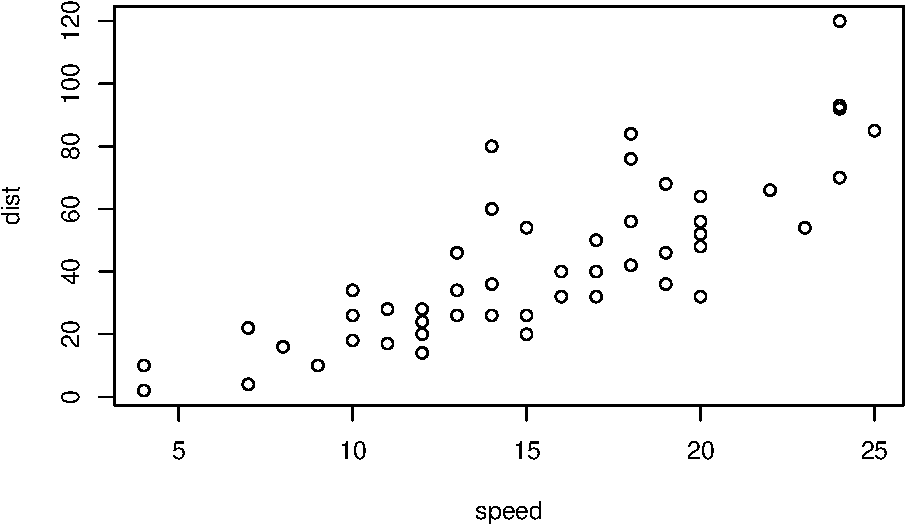
\includegraphics{_main_files/figure-latex/figure-label-1.pdf}
\caption{\label{fig:figure-label}A sample figure}
\end{figure}

\begin{Shaded}
\begin{Highlighting}[]
\NormalTok{See Figure \textbackslash{}@ref(fig:figure{-}label) for the graph.}
\end{Highlighting}
\end{Shaded}

\begin{center}\rule{0.5\linewidth}{0.5pt}\end{center}

\section{Tips for LaTeX in Bookdown}\label{tips-for-latex-in-bookdown}

\begin{enumerate}
\def\labelenumi{\arabic{enumi}.}
\item
  \textbf{Use Labels Consistently}: Use meaningful and unique labels for cross-referencing.
\item
  \textbf{Use Math Mode}: Always enclose mathematical symbols in \texttt{\$...\$} or \texttt{\$\$...\$\$} to render correctly.
\item
  \textbf{Add Theorem Styles}: Customize theorem environments in \texttt{\_bookdown.yml} for specific needs:

\begin{Shaded}
\begin{Highlighting}[]
\FunctionTok{theorem}\KeywordTok{:}
\AttributeTok{  }\FunctionTok{lab}\KeywordTok{:}\AttributeTok{ }\StringTok{"Theorem "}
\AttributeTok{  }\FunctionTok{lem}\KeywordTok{:}\AttributeTok{ }\StringTok{"Lemma "}
\end{Highlighting}
\end{Shaded}
\item
  \textbf{Install Necessary Packages}: Ensure you have a LaTeX distribution installed (e.g., TinyTeX).
\end{enumerate}

\begin{center}\rule{0.5\linewidth}{0.5pt}\end{center}

This tutorial should provide a strong foundation for using LaTeX in your Bookdown projects. With these tools, you can create professional, structured, and highly readable documents.

\chapter{LaTeX Distributions}\label{latex-distributions}

To render PDF outputs with Bookdown, you need to install a LaTeX distribution. Below is a list of popular options, categorized by operating system and user preferences:

\section{Recommended LaTeX Distribution}\label{recommended-latex-distribution}

\subsection{\texorpdfstring{1. \textbf{TinyTeX} (Recommended)}{1. TinyTeX (Recommended)}}\label{tinytex-recommended-1}

\begin{itemize}
\item
  \textbf{Description}: A lightweight, cross-platform LaTeX distribution designed to work seamlessly with R and Bookdown.
\item
  \textbf{Installation}: Run the following commands in R:

\begin{Shaded}
\begin{Highlighting}[]
\FunctionTok{install.packages}\NormalTok{(}\StringTok{"tinytex"}\NormalTok{)}
\NormalTok{tinytex}\SpecialCharTok{::}\FunctionTok{install\_tinytex}\NormalTok{()}
\end{Highlighting}
\end{Shaded}
\item
  \textbf{Advantages}:

  \begin{itemize}
  \tightlist
  \item
    Minimal installation size.
  \item
    Automatically installs missing packages when rendering.
  \end{itemize}
\item
  \textbf{Website}: \href{https://yihui.org/tinytex/}{TinyTeX Documentation}
\end{itemize}

\begin{center}\rule{0.5\linewidth}{0.5pt}\end{center}

\section{Additional LaTeX Distributions}\label{additional-latex-distributions-1}

\subsection{\texorpdfstring{2. \textbf{TeX Live}}{2. TeX Live}}\label{tex-live-1}

\begin{itemize}
\tightlist
\item
  \textbf{Description}: A comprehensive LaTeX distribution suitable for Linux and cross-platform users.
\item
  \textbf{Installation}:

  \begin{itemize}
  \item
    \textbf{Linux}:

\begin{Shaded}
\begin{Highlighting}[]
\FunctionTok{sudo}\NormalTok{ apt{-}get install texlive{-}full}
\end{Highlighting}
\end{Shaded}
  \item
    \textbf{macOS and Windows}: Download from \href{https://www.tug.org/texlive/}{TeX Live}.
  \end{itemize}
\item
  \textbf{Advantages}:

  \begin{itemize}
  \tightlist
  \item
    Full-featured with a vast collection of LaTeX packages.
  \item
    Stable and widely used.
  \end{itemize}
\item
  \textbf{Website}: \href{https://www.tug.org/texlive/}{TeX Live Documentation}
\end{itemize}

\begin{center}\rule{0.5\linewidth}{0.5pt}\end{center}

\subsection{\texorpdfstring{3. \textbf{MikTeX}}{3. MikTeX}}\label{miktex-1}

\begin{itemize}
\tightlist
\item
  \textbf{Description}: A user-friendly LaTeX distribution popular among Windows users.
\item
  \textbf{Installation}: Download and install from \href{https://miktex.org/}{MikTeX}.
\item
  \textbf{Advantages}:

  \begin{itemize}
  \tightlist
  \item
    On-demand installation of missing packages.
  \item
    Easy-to-use package manager.
  \end{itemize}
\item
  \textbf{Website}: \href{https://miktex.org/}{MikTeX Documentation}
\end{itemize}

\begin{center}\rule{0.5\linewidth}{0.5pt}\end{center}

\subsection{\texorpdfstring{4. \textbf{MacTeX} (for macOS)}{4. MacTeX (for macOS)}}\label{mactex-for-macos-1}

\begin{itemize}
\tightlist
\item
  \textbf{Description}: A macOS-specific version of TeX Live with additional tools for macOS users.
\item
  \textbf{Installation}: Download and install from \href{https://www.tug.org/mactex/}{MacTeX}.
\item
  \textbf{Advantages}:

  \begin{itemize}
  \tightlist
  \item
    Tailored for macOS with GUI tools like TeXShop.
  \item
    Includes a full TeX Live distribution.
  \end{itemize}
\item
  \textbf{Website}: \href{https://www.tug.org/mactex/}{MacTeX Documentation}
\end{itemize}

\begin{center}\rule{0.5\linewidth}{0.5pt}\end{center}

\subsection{\texorpdfstring{5. \textbf{ProTeXt} (for Windows)}{5. ProTeXt (for Windows)}}\label{protext-for-windows-1}

\begin{itemize}
\tightlist
\item
  \textbf{Description}: A Windows-specific distribution that combines MikTeX with a user-friendly installer.
\item
  \textbf{Installation}: Download and install from \href{https://www.tug.org/protext/}{ProTeXt}.
\item
  \textbf{Advantages}:

  \begin{itemize}
  \tightlist
  \item
    Streamlined setup for beginners.
  \item
    Integrates LaTeX editors like TeXworks.
  \end{itemize}
\item
  \textbf{Website}: \href{https://www.tug.org/protext/}{ProTeXt Documentation}
\end{itemize}

\begin{center}\rule{0.5\linewidth}{0.5pt}\end{center}

Choose the distribution that best fits your operating system and needs. For most users, TinyTeX is the easiest to install and manage, especially if you're using R and Bookdown.

  \bibliography{book.bib}

\end{document}
